\section{Rate Selection using SNR in Practice}
As a baseline measurement, I analyze the accuracy of the Packet SNR estimate computed from RSSI when used to select rates over wireless links. This algorithm gathers the Packet SNR $\rho$ and then returns the fastest working MCS (\algref{alg:rate_select_snr}).

%%%%%%%%%%%%%%%%%%%%%%%%%%%%%%%%%%%%%%%%%%%%%%%%
\begin{algorithm}[t]
\caption{\label{alg:rate_select_snr}\fcall{SelectRateSnr($\text{Sender }s, \text{Receiver }r$)}}
\begin{algorithmic}
\STATE $s$ sends a packet, either a probe packet with no payload or a normal data packet
\STATE $r$ computes the SNR $\rho$ of the received packet and feeds it back to $s$ with the ACK
\IF{$s$ does not receive an ACK}
\RETURN $-1$ \hfill \COMMENT{indicating failure; could use the prior estimate or try again}
\ELSE
\RETURN {$\argmax_m \fcall{GetBitrateThreshold}(m, \rho, \tau_m)$} \hfill \COMMENT{fastest working MCS}
\ENDIF
\end{algorithmic}
\end{algorithm}

\begin{algorithm}[t]
\caption{\label{alg:get_bitrate_threshold}\fcall{GetBitrateThreshold(MCS $m$, SNR $\rho$, Threshold $\tau$)}}
\begin{algorithmic}
\IF{$\rho > \tau$}
\RETURN {the bit rate of \mcs{$m$}} \hfill \COMMENT{\mcs{$m$} works}
\ELSE
\RETURN {0} \hfill \COMMENT{\mcs{$m$} does not work}
\ENDIF
\end{algorithmic}
\end{algorithm}

\begin{algorithm}[t]
\caption{\label{alg:predict_rate_snr}\fcall{PredictBitrateSnr($\text{Sender }s, \text{Receiver }r$)}}
\begin{algorithmic}
\STATE $s$ sends a packet, either a probe packet with no payload or a normal data packet
\STATE $r$ computes the SNR $\rho$ of the received packet and feeds it back to $s$ with the ACK
\IF{$s$ receives an ACK from $r$}
\RETURN \fcall{SnrToThroughput($\rho$)}
\ELSE
\RETURN $0$ \hfill \COMMENT{indicating failure; could use the prior estimate or try again}
\ENDIF
\end{algorithmic}
\end{algorithm}
%%%%%%%%%%%%%%%%%%%%%%%%%%%%%%%%%%%%%%%%%%%%%%%%

\subsection{Computing SNR Thresholds}
Note that \algref{alg:rate_select_snr} requires an SNR threshold $\tau_m$ for every \mcs{$m$} to determine if that rate is supported. If SNR accurately reflected the rate of the channel, we could use the SNR thresholds measured over a wired link, e.g., as shown in \figref{fig:snr_prr_attenuator}. As this does not work in practice, I computed these thresholds empirically by measuring wireless links in my testbeds.

I measured the relation between SNR and PRR while varying the transmit power level, and hence the received SNR, for each single-antenna rate (\mcs{0}--\mcs{7}). These measurements cover 202 indoor, single-antenna wireless links from both 802.11n testbeds.
%Not all pairs in all testbeds successfully deliver any packets at all.
For each \mcs{$m$} on each link, I determined the SNR level at \mcs{$m$} resulted in more throughput than the next lower rate. For example, \mcs{2} has a bit rate of 19.5\Mbps while \mcs{1} has a bit rate of 13\Mbps, so the SNR threshold for \mcs{2} should be the SNR value at which the link can deliver at least 2/3 of the transmitted packets.

\begin{figure}[ht]
	\centering
	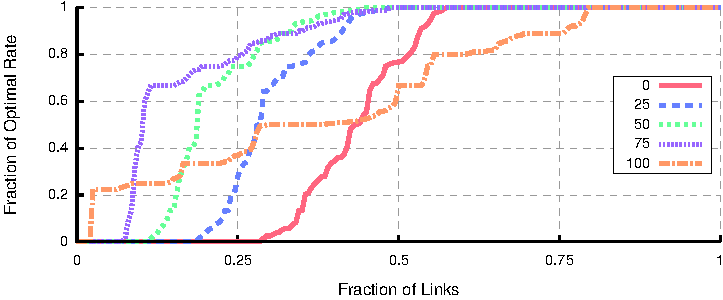
\includegraphics[width=\textwidth]{figures/thresh_vs_opt.pdf}
	\caption[The accuracy of selecting rate using SNR for thresholds derived from differing percentiles of the transition region.]{\label{fig:thresh_vs_opt}The accuracy of selecting rate using SNR for thresholds derived from differing percentiles of the transition region. [XXXNote: I think this data is a bit wrong, and need to revisit]}
\end{figure}

This process results in a different threshold for each MCS for each link; however we need one threshold that works well across links. To choose such a threshold, I can select some percentile of this set. Using low SNR thresholds (near the 0th percentile) gives an aggressive rate selection algorithm, that will perform sub-optimally for many links because it sends packets too fast to be received. Conversely, a conservative algorithm will choose high SNR thresholds (near the 100th percentile), leading to sub-optimal performance as packets are sent slower than necessary.

\subsection{Results}
\figref{fig:thresh_vs_opt} shows the relationship between threshold and performance for the 202 measures links. We see that no threshold---aggressive, conservative, or somewhere in the middle---provides good performance across the range of real wireless links. The best-performing threshold is probably about the 75th percentile. Despite being a relatively conservative choice, this threshold provides near-optimal performance for half of links, and only about 1 in 10 links suffers dramatically from over-selected rates.

Finally, this figure shows room for improvement in rate selection, and illustrates why SNR-based rate selection in its pure form has never been used for 802.11. 

